\documentclass{beamer}
\usetheme{Boadilla}
\usepackage{bibentry}
\usepackage{cmbright}
\usepackage{natbib}
\setbeamertemplate{itemize items}[circle]
\setbeamertemplate{enumerate items}[default]

\def\E{\text{E}}
\def\Var{\text{Var}}
\def\Cov{\text{Cov}}

\title[Euler Equations]{Work in Progress: The Euler Equation Implied Rate Under Heterogeneous Preferences}
\author[Li]{Pearl Li}
\date{November 18, 2015}

\begin{document}

\begin{frame}
\titlepage
\end{frame}


\begin{frame}{Literature}
\begin{itemize}
\item \cite{hara09}: aggregating heterogeneous discount rates and risk attitudes into a representative agent
\item \cite{tesfatsion05}: agent-based computational modeling
\end{itemize}
\end{frame}

\begin{frame}{Raw Data}
\begin{itemize}
\item Quarterly data from 1960:Q1 to 2015:Q2 \bigskip
\item FRED (Federal Reserve Economic Data from the St. Louis Fed)
  \begin{itemize}
  \item Civilian noninstitutional population
  \item Effective fed funds rate
  \item Employment ratio
  \item Weekly hours worked (non-farm)
  \item Nominal consumption of nondurable goods
  \item Nominal consumption of services
  \item Real disposable income
  \item Real GDP
  \item Chain quantity index: nondurable goods
  \item Chain quantity index: services
  \end{itemize}
\item Continuous Commodity Index
\end{itemize}
\end{frame}

\begin{frame}{Generated Series}
\begin{itemize}
\item $\text{Nominal consumption}_t = \text{nondurable goods}_t + \text{services}_t$
\item $\text{Real consumption}_t \text{ (in chained 2009 dollars)} = \text{2009 nominal consumption} \times \text{chain quantity index}_t$
\item $\text{Consumption deflator}_t = \frac{\text{nominal consumption}_t}{\text{real consumption}_t}$
\item $\text{Gross inflation}_t = \frac{\text{consumption deflator}_t}{\text{consumption deflator}_{t-1}}$
\item $\text{Labor fraction}_t = \text{hours worked}_t \times \text{employment ratio}_t$, rescaled to have mean $\frac{1}{3}$
\item $\text{Leisure fraction}_t = 1 - \text{labor fraction}_t$ \bigskip\bigskip
\item Most series following \cite{collard11}
\end{itemize}
\end{frame}

\begin{frame}{VAR Model}
\begin{itemize}
\item Estimate VAR(4) (written below in companion form)
\item Lag order 4 chosen for optimal likelihood ratio --- as in \cite{fuhrer00}, \cite{collard11}
\end{itemize}
$$y_t = A_0 + A_1 Y_{t-1} + \nu_t$$
$$\nu_t \overset{\text{iid}}{\sim} N(0, \Sigma)$$
\begin{align*}
y_t &= \begin{bmatrix} \log(\text{real consumption}_t) \\ \text{net inflation}_t \\ \text{leisure fraction}_t \\ \log(\text{real disposable income}_t) \\ \log(\text{income less consumption}_t) \\ \text{effective FFR}_t \\ \text{CCI}_t \end{bmatrix} &
Y_t &= \begin{bmatrix} y_t \\ y_{t-1} \\ y_{t-2} \\ y_{t-3} \end{bmatrix}
\end{align*}
\end{frame}

\begin{frame}{VAR Estimates}
\begin{itemize}
\item Sample: 1960:Q2 to 2015:Q2 (221 observations)
\item Log likelihood: 2282.281
\item Ljung-Box statistic: 4544.5290 ($p$-value 0.0000) \bigskip
\item Conditional moments:
  \begin{itemize}
  \item $\E_t Y_{t+1} = A_0 + A_1 Y_t$
  \item $\Cov_t Y_{t+1} = \hat{\Sigma}$
  \end{itemize}
\end{itemize}
\end{frame}

\begin{frame}{CRRA Implied Rates}
\begin{itemize}
\item CRRA utility $u(C_t) = \frac{C_t^{1-\alpha}}{1-\alpha}$
\item Euler equation $\frac{1}{1+r_t} = \beta \frac{E_t u'(C_{t+1})}{u'(C_t)} = \beta \left( \frac{\E_t C_{t+1}}{C_t} \right)^{-\alpha}$
\item From \cite{canzoneri07}: assuming consumption is conditionally lognormal, real interest rate given by
$$\frac{1}{1+r_t} = \beta \exp\left[ -\alpha(\E_t c_{t+1} - c_t) + \frac{\alpha^2}{2} \Var_t c_{t+1} \right]$$ where $c_t$ is log of real consumption $C_t$
\item $\beta = 0.9926$, $\alpha = 2$ as in \cite{collard11}
\end{itemize}
\end{frame}

\begin{frame}{CRRA Implied Rates}
\begin{center}
\begin{tabular}{cc}
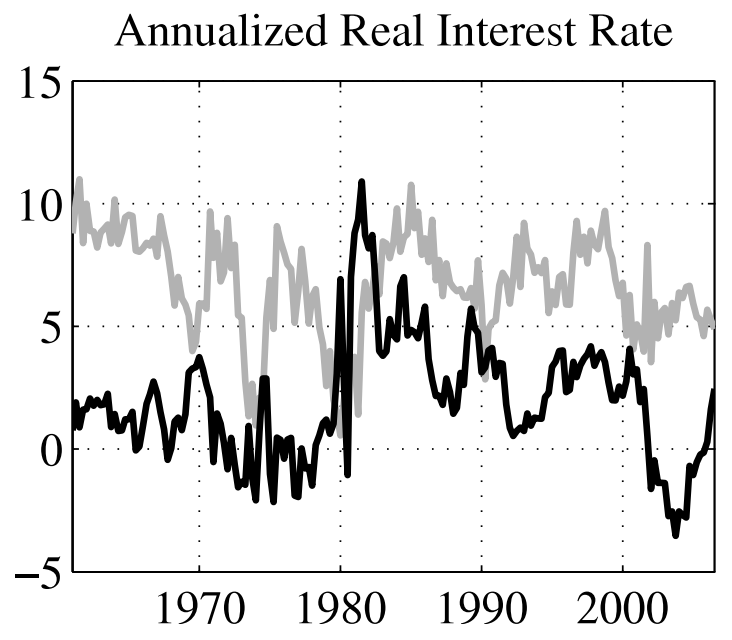
\includegraphics[height=120px]{crra-real_collard.png} &
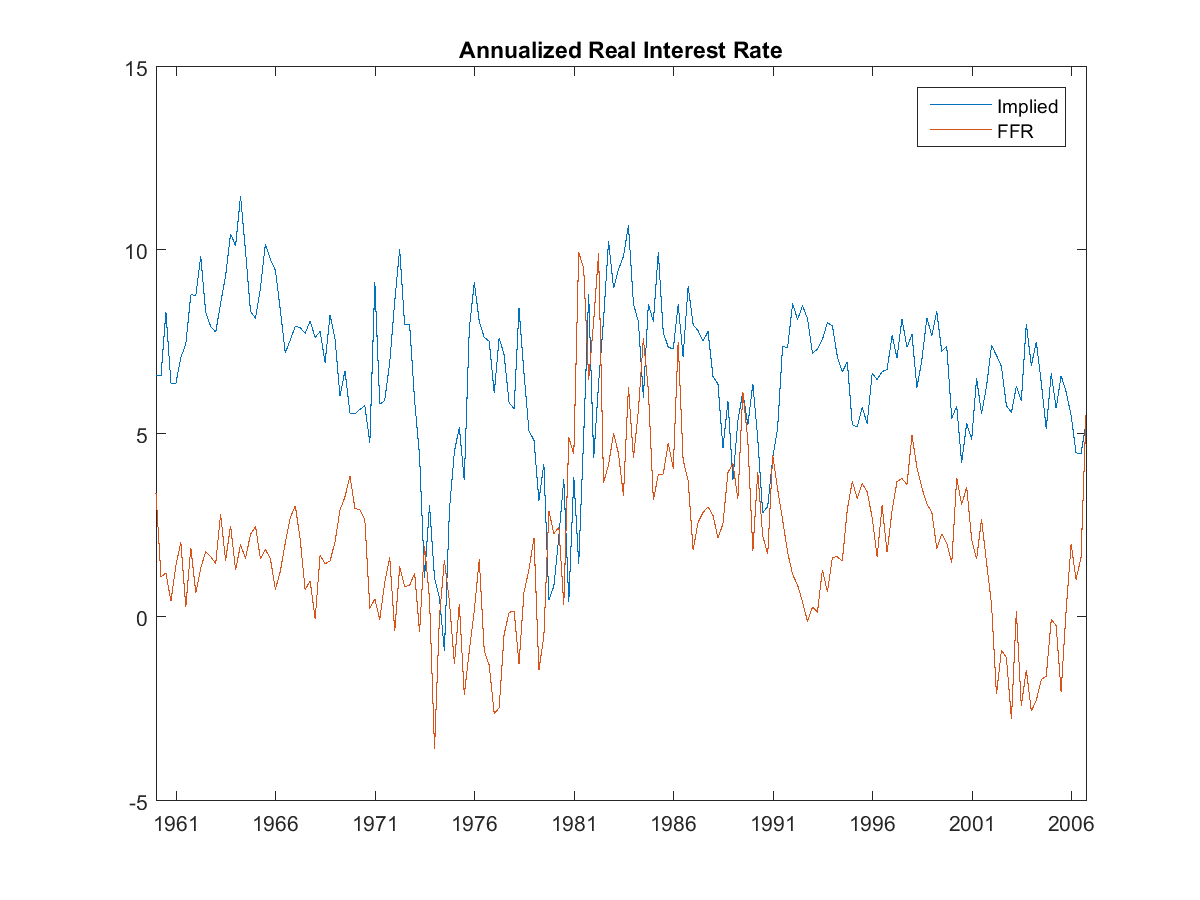
\includegraphics[height=120px]{crra-real.png} \\
\cite{collard11} & Li (2015) \\
(gray = implied, black = FFR) & 
\end{tabular}
\end{center}
\end{frame}

\begin{frame}{CRRA Implied Rates}
\begin{center}
\begin{tabular}{|l|l|l|} \hline
                  & \cite{collard11} & Li (2015) \\ \hline
Mean implied rate & 6.70             & 6.66      \\ \hline
SD implied rate   & 2.09             & 2.13      \\ \hline
Mean FFR          & 1.99             & 1.98      \\ \hline
SD implied rate   & 2.51             & 2.30      \\ \hline
Correlation       & 0.05             & 0.0146    \\ \hline
\end{tabular}
\end{center}
\end{frame}

\begin{frame}{Problems}
\begin{center}
\begin{tabular}{cc}
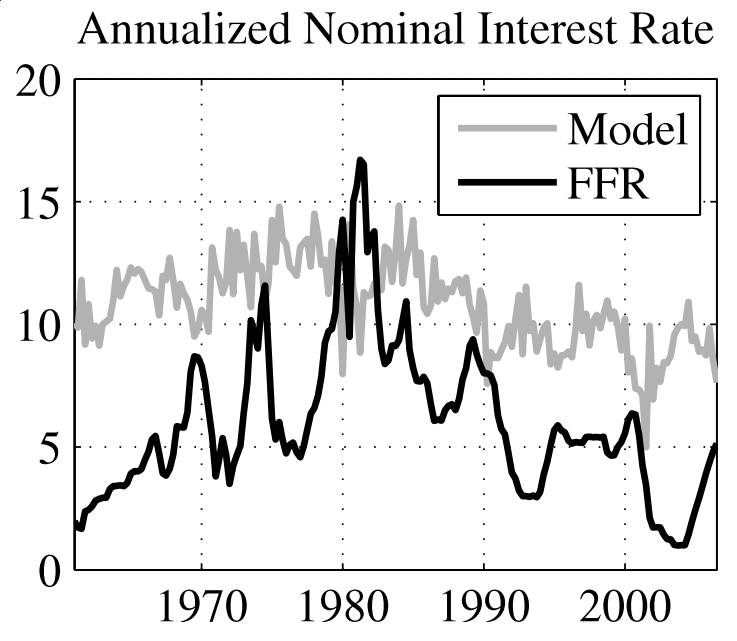
\includegraphics[height=120px]{crra-nominal_collard.png} &
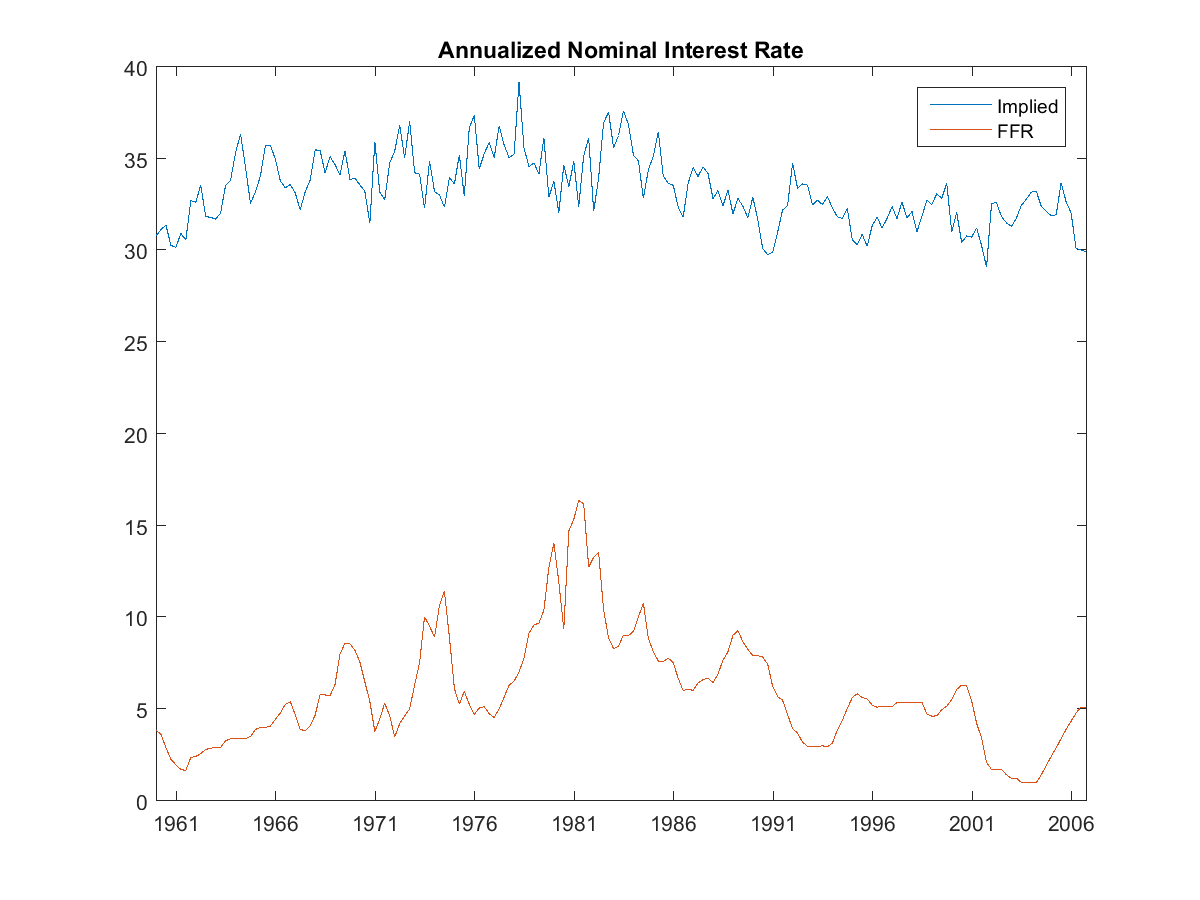
\includegraphics[height=120px]{crra-nominal.png} \\
\cite{collard11} & Li (2015)
\end{tabular}
\end{center}
\end{frame}

\begin{frame}{To Come}
\begin{itemize}
\item Why are computed nominal implied rates so high?
\item Implied rates with habit formation and consumption/leisure non-separability
\item Impulse responses to monetary shock
\item Monte Carlo experiment
\item \textbf{Heterogeneous preferences}
\end{itemize}
\end{frame}

\begin{frame}{References}
\bibliographystyle{../refs/econ}
\bibliography{../refs/refs}
\end{frame}

\end{document}